\chapter{Sequenzer}
\label{ch:Sequenzer}
\section{Allgemeines}
Bei dieser Umsetzung eines Sequenzers wurde sich für maximal fünf alternierende Spannungspegel entschieden. In der Literatur ist diese Unterart als 5-Step-Sequencer bekannt, welcher wegen seiner markanten Charakteristik zum Beispiel auch im bekannten 'Buchla Easel Command ECM-X7' Synthesizer verbaut ist. Über zwei in der Handebene verbaute Kippschalter kann alternativ zwischen 3- bzw. 4-Stufen-Betrieb gewählt werden. Welcher Schritt aktuell aktiv ist wird durch Status-LEDs in der Frontplatte angezeigt.\\
Als Spannungsversorgung erhält der Sequenzer \textpm 12 Volt durch das verbaute Netzteil. Optional kann ein externes Clock-Signal, beispielsweise von einem LFO (vgl. Kapitel \ref{ch:LFO}), angeschlossen werden. Der eigene Takt wird dadurch überbrückt, wodurch das Modul flexibel eingesetzt werden kann. Des Weiteren kann die Sequenz durch ein externes Signal zurückgesetzt werden. Dadurch wird automatisch wieder bei der ersten Stufe der Sequenz begonnen, wodurch dem Nutzer weiterer musikalischer Freiraum freigeräumt wird.\\
Das Sequenzer-Modul verfügt über drei abgreifbare Ausgangssignale. Ein Clock-Signal, welches über ein Potentiometer in der Handebene parametrisiert werden kann, gibt den internen Takt des Moduls vor, und kann von außerhalb abgegriffen werden. Dessen Spannung toggelt dabei zwischen -12 und +12 Volt. Die Control Voltage (CV) wird zumeist dem VCO (vgl. Kapitel \ref{ch:VCO}) zur weiteren Verarbeitung überreicht. Dabei handelt es sich um eine alternierende Spannungsfolge, welche zwischen 0 und 5 Volt schwanken kann. Die einzelnen Spannungspegel der bis zu fünf Stufen werden durch ein jeweiliges Potentiometer in der Handebene eingestellt. Das dritte Ausgangssignal des Sequenzers bildet der Gate. Ähnlich dem CV wird eine alternierende Spannungsfolge von bis zu fünf Stufen ausgegeben, wobei eine Stufe in zwei Abschnitte geteilt wird. Der erste Abschnitt beträgt, abhängig dem jeweiligen Kippschalter in der Handebene, entweder +12 oder 0 Volt. Der zweite Abschnitt führt immer 0 Volt. Der Gate verhält sich somit ähnlich dem Clock-Signal. Er führt jedoch niemals eine Negative Spannung und seine Stufen sind manuell zuschaltbar. In der Regel wird der Gate als Eingangssignal für den ADSR hergenommen.

\section{Schaltplan}
\newpage	%Seite leer beenden und Umbruch


%\begin{figure}[h]
%	\centering
%	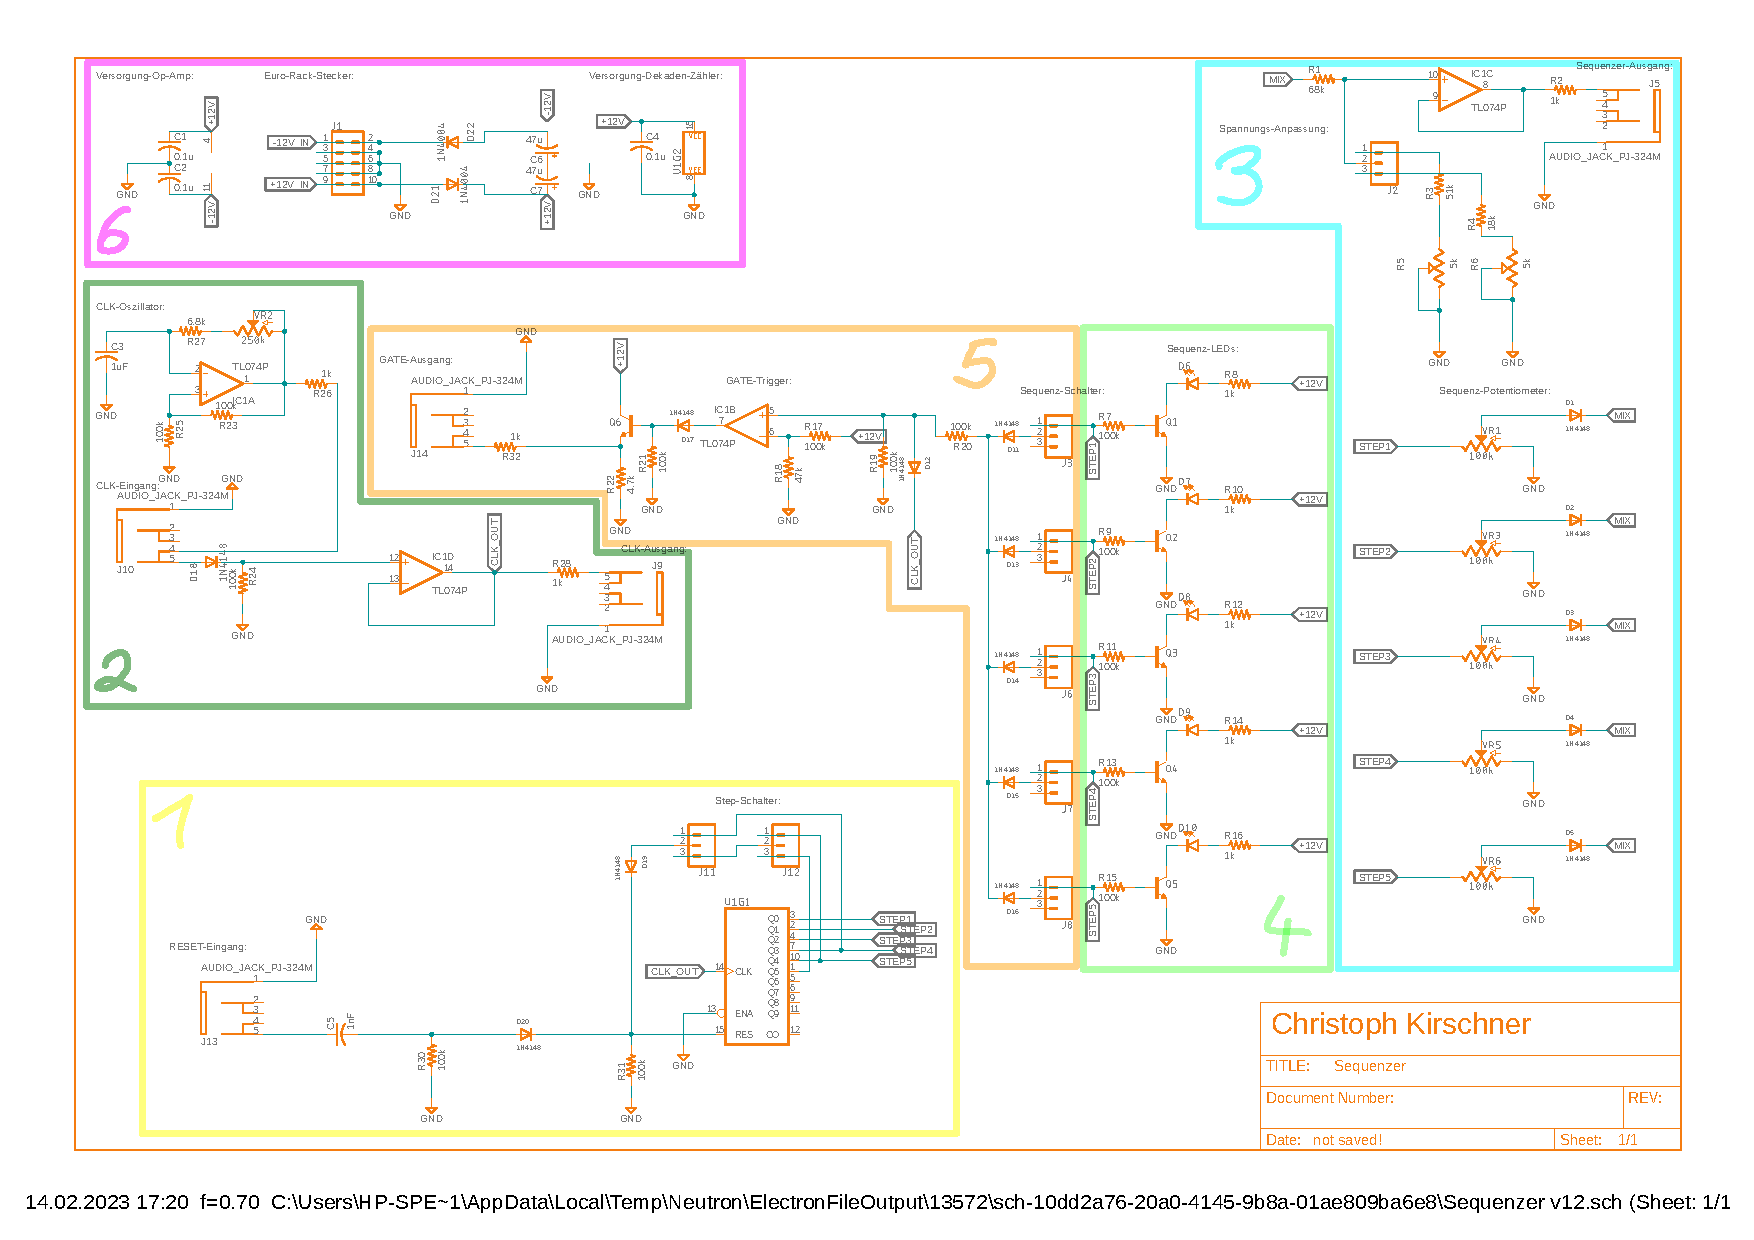
\includepdf[angle=270, clip, trim=1.7cm 0.85cm 0.8cm 1.65cm, scale=0.8] {figures/Schaltplan_Sequenzer_Christoph_Kirschner_unterteilt.pdf}
%	\caption{Schaltplan der Sequenzer-Platine}
%	\label{fig:Schaltplan_des_Sequenzers}
%\end{figure}
%\FloatBarrier
%\newpage	%Seite leer beenden und Umbruch

\begin{figure}[h]
	\centering
	\setlength{\fboxsep}{1pt} %Abstand der Linien zur Abbildung
	\setlength{\fboxrule}{1pt} %Dicke der Linie
	\fbox{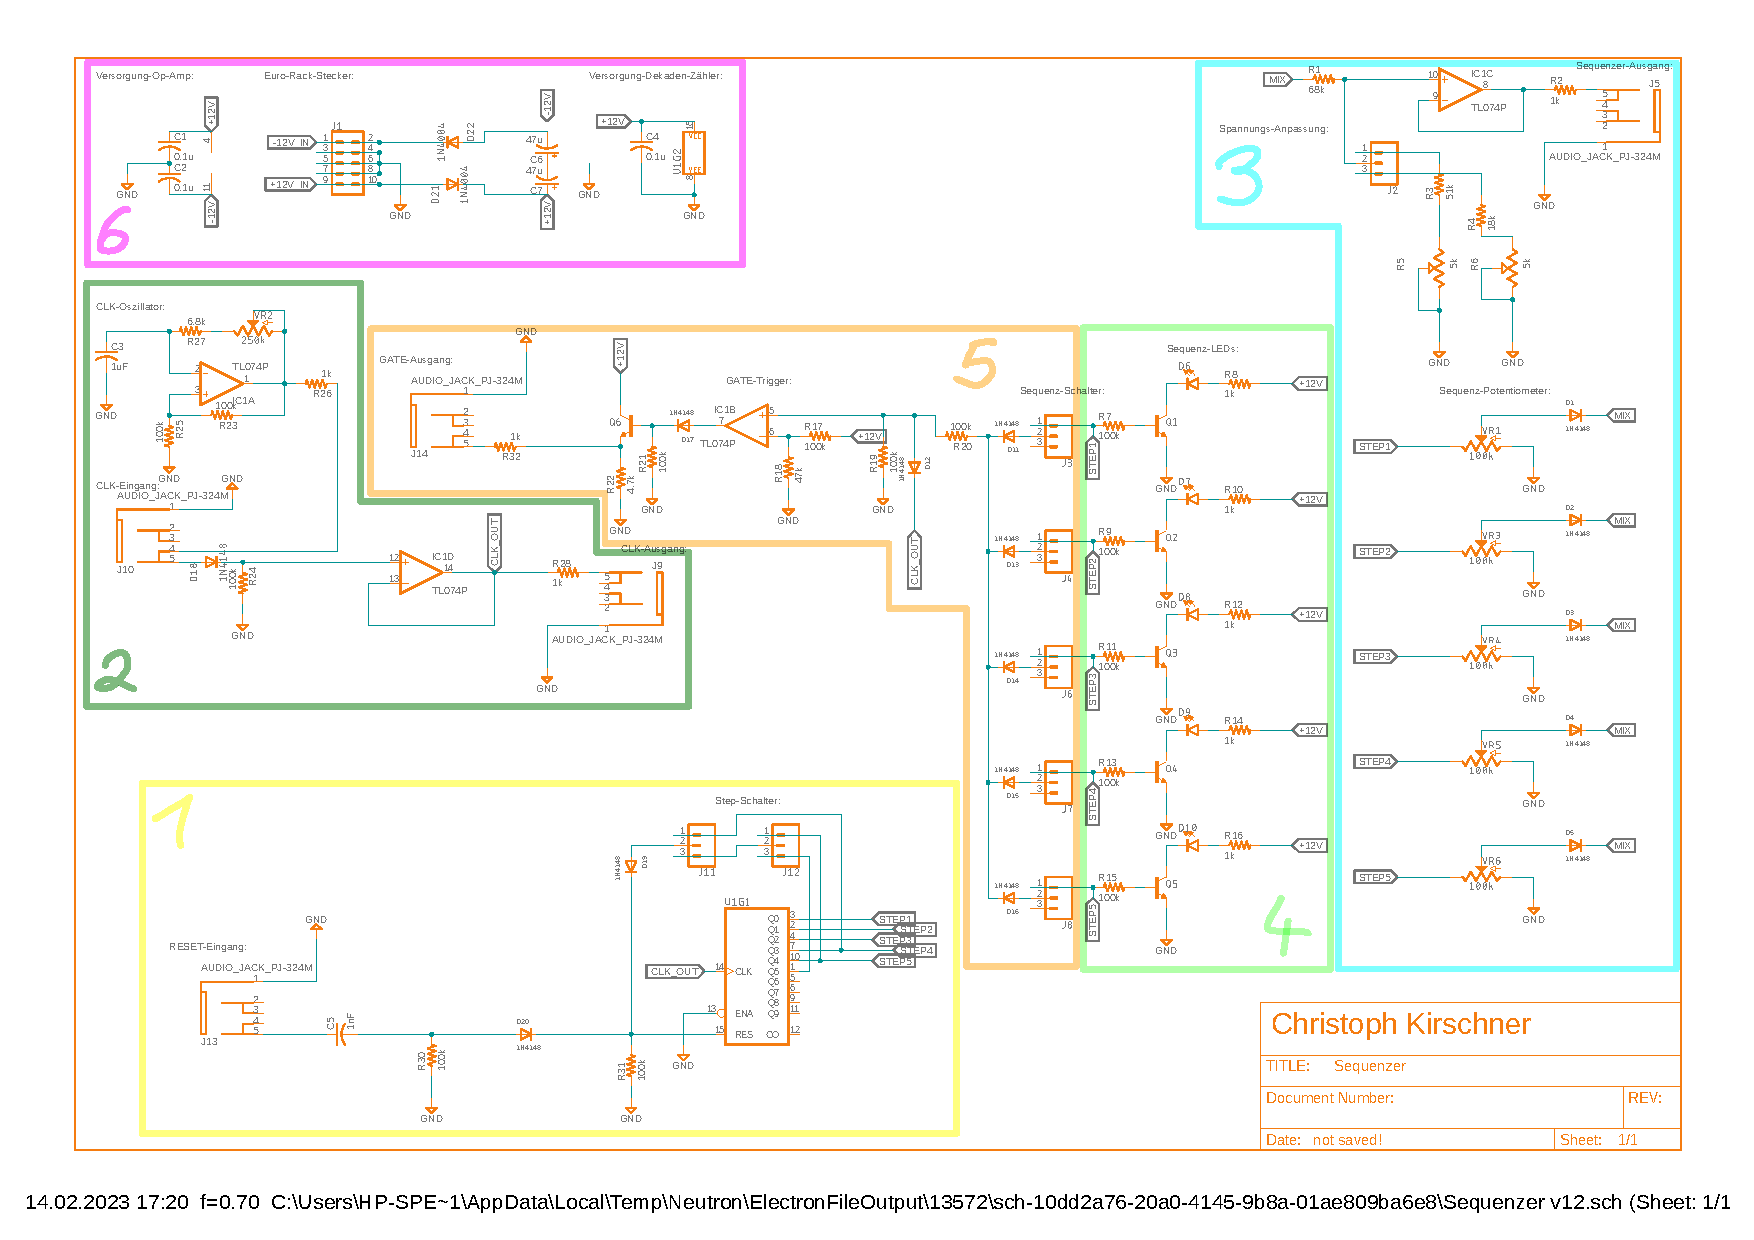
\includegraphics[angle=270, clip, trim=1.25cm 1.48cm 1.20cm 0.95cm, scale=0.8, width=1\textwidth] {figures/Schaltplan_Sequenzer_Christoph_Kirschner_unterteilt.pdf}}
	\caption{Schaltplan der Sequenzer-Platine}
	\label{fig:Schaltplan_des_Sequenzers}
\end{figure}
\FloatBarrier
\newpage	%Seite leer beenden und Umbruch

Der Schaltplan des Sequenzers lässt sich, wie in Abbildung \ref{fig:Schaltplan_des_Sequenzers} gezeigt, in sechs Bereiche unterteilen. Der Bereich eins ist zuständig für das Durchschalten der Zustände.
Die wesentliche Komponente ist dabei das Bauteil U1G1. Es handelt sich dabei um einen CD4017 Dekadenzähler, der durch das Toggeln des Clock-Signals die verschiedenen Zustände durchschaltet. Der Sequenzer ist für eine Sequenz von maximal 5 Stufen ausgelegt. Durch die beiden Schalter J11 und J12 kann diese jedoch auf 4 bzw. 3 Stufen reduziert werden, was sich an der Rückführung der jeweiligen Stufen auf den RESET-Pin erkennen lässt. Durch den RESET-Eingang J13 lässt sich zusätzlich ein externes Signal einbinden, was einen Fremd-RESET ermöglicht.\\
Der zweite Bereich des Schaltplans kümmert sich um das Clock-Signal. Dafür wird der Operationsverstärker (OPV) IC1A sowohl über eine Mitkopplung durch R23, als auch über eine Gegenkopplung durch R27 und VR2 betrieben. Der dadurch realisierte Negativ-Impedanz-Konverter läd bzw. entläd den Kondensator C3 in Abhängigkeit des Potentiometers VR2. Das daraus entstehende Clock-Signal wird über einen Buffer (IC1D) geführt und unter anderem über den Klinkenausgang J9 nach außen zur Verfügung gestellt. Der Klinkeneingang J10 ist zusätzlich in der Lage das interne Clock-Signal durch ein extern angelegtes zu übersteuern.\\
Im dritten Abschnitt werden den verschieden Zuständen ihre jeweiligen Spannungen zugewiesen. Um das zu erreichen wird jedes Zustandssignal über ein separates Potentiometer gegen Masse geführt. Der Abgriff wird anschließend durch jeweilige Dioden vor rückfließenden Strömen geschützt und zusammengeführt. Um das Spannungssignal nun zu limitieren, wurden zwei Spannungsteiler R1 und R3 für 0 - 5 Volt sowie R1 und R4 für 0 - 2.5 Volt eingesetzt. Um Bauteiltoleranzen kompensieren zu können wurden zusätzlich zwei Trimmer R5 und R6 verbaut. Zwischen den Spannungsbereichen kann über den Schalter J2 gewechselt werden (default: 0 - 5 Volt). Danach kommt wieder ein Buffer (IC1C) und in Reihe dazu der Widerstand R2. Dieser Widerstand sorgt dafür, dass im Falle eines Kurzschlusses der Fehlerstrom begrenzt und dadurch kein Schaden in der Schaltung entsteht. Der so entstandene CV kann über den Klinkenausgang J5 abgegriffen werden.\\
Der vierte Bereich des Schaltplans (vgl. Abbildung \ref{fig:Schaltplan_des_Sequenzers}) ermöglicht das Ablesen des aktiven Zustandes über die Frontplatte. 
Dafür wird für jeden möglichen Zustand eine LED (D6 - D10) angeschaltet, welche nach außen geführt ist. 
Die LEDs werden durch eine Emitterschaltung eines 2N3904 NPN Transistor angesteuert. Somit werden die Spannungssignale entlastet und möglichem Schaden vorgebeugt.\\
Die Funktionalität des Gate-Ausgangs wird in Bereich fünf umgesetzt. Die verschiedenen Stufenspannungen des Dekadenzählers aus Bereich eins werden jeweils über einen Kippschalter sowie eine Diode geführt und danach vereint. Die Schalter ermöglichen ein manuelles Zu- bzw. Wegschalten der einzelnen Stufe im resultierenden Gate-Signal. Die Dioden verhindern, wie auch bei der Umsetzung des CV, ein rückfließen der Ströme in die anderen Stufensignale. Nach der Zusammenführung der Signale folgt der Widerstand R20, sowie das über eine Diode begrenzte Clock-Signal. Das Clock-Signal sorgt dafür das der Gate in jedem Zyklus für die halbe Zeit auf 0 Volt gesetzt wird. Durch den Widerstand R20 wird einem Kurzschluss in diesem Pfad vorgebeugt. Der Widerstand R19 verhindert einen undefinierten Zustand sobald ein Stufe durch einen Kippschalter weggeschaltet wird. Allerdings bilden R19 und R20 einen ungewollten Spannungsteiler, der aus den gewünschten +12 Volt +6 Volt macht. Aus diesem Grund wurde ein weiterer OPV als einfacher Komparator verbaut. Die Widerstände R17 und R18 sorgen für eine Vergleichsspannung von 3.8 Volt am nicht-invertierenden Eingang, weshalb bei den anliegenden +6 Volt problemlos durchgeschaltet wird. Der negative Teil der Spannung wird anschließend durch die Diode D17 sowie den Pulldown-Widerstand R21 unterbunden. Um der resultierenden hohen Impedanz sowie der begrenzt möglichen Stromentnahme der aktuellen Schaltung entgegenzuwirken, wurde der Ausgang mit einem BC547 NPN Transistor versehen. Dieser wurde als Kollektorschaltung implementiert sowie, um Kurzschlüsse zu vermeiden, mit einem weiteren Widerstand R32 verbaut. Der Gate kann somit über den Klinkenausgang J14 von außen abgegriffen werden.\\
Der letzte Bereich ist zuständig für die Spannungsversorgung des gesamten Moduls. Das Netzteil (vgl. Kapitel \ref{ch:Netzteil}) versorgt den Sequenzer mit \textpm 12 Volt durch den Euro-Rack-Stecker. Um Verpolung vorzubeugen, wurden zwei Dioden D21 und D22 verbaut. Anschließend werden die beiden Spannungen mit den Kondensatoren C6 und C7 gegen Masse gepuffert. Weitere Pufferkondensatoren wurden in der Versorgung der OPV als auch in der Versorgung des Dekadenzählers vorgesehen \cite{seq_manual}.

\section{Platine}
\begin{figure}[h]
	\centering
	\setlength{\fboxsep}{1pt} %Abstand der Linien zur Abbildung
	\setlength{\fboxrule}{1pt} %Dicke der Linie
	\fbox{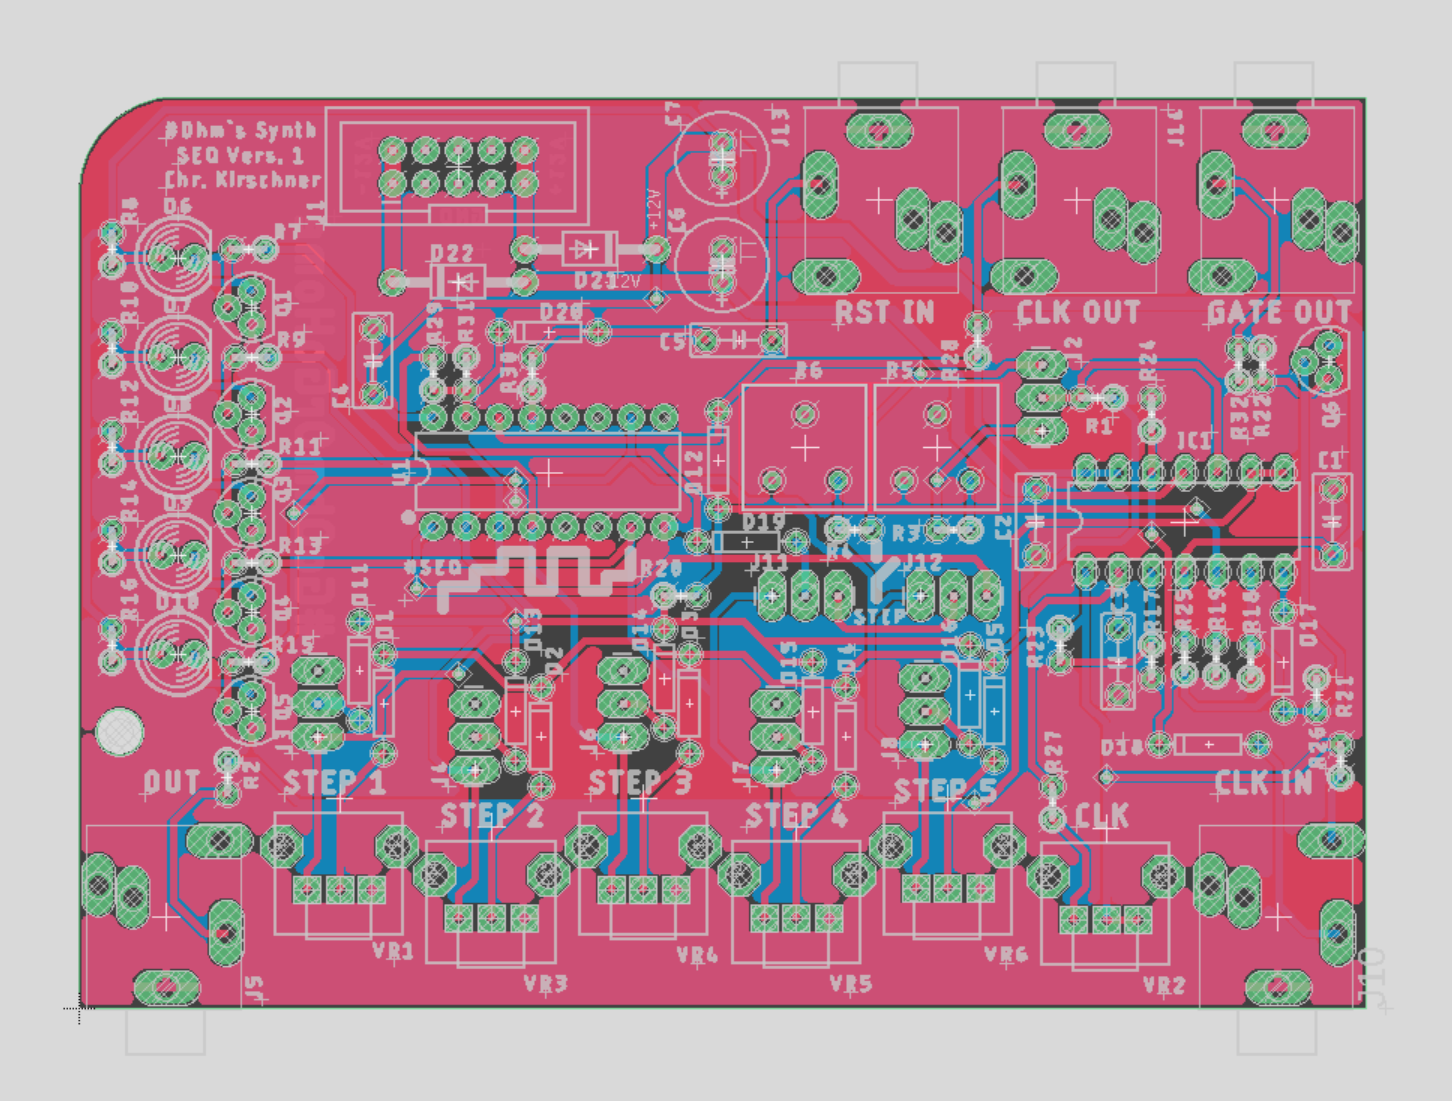
\includegraphics[width=1\textwidth]{figures/Sequenzer_Layout.PNG}}
	\caption{Ausschnitt des Sequenzer-Platinen-Layouts aus Fusion360}
	\label{fig:PCB_SEQ}
\end{figure}
\FloatBarrier
\newpage

\section{Mechanischer Aufbau}
\begin{figure}[h]
	\centering
	\setlength{\fboxsep}{1pt} %Abstand der Linien zur Abbildung
	\setlength{\fboxrule}{1pt} %Dicke der Linie
	\fbox{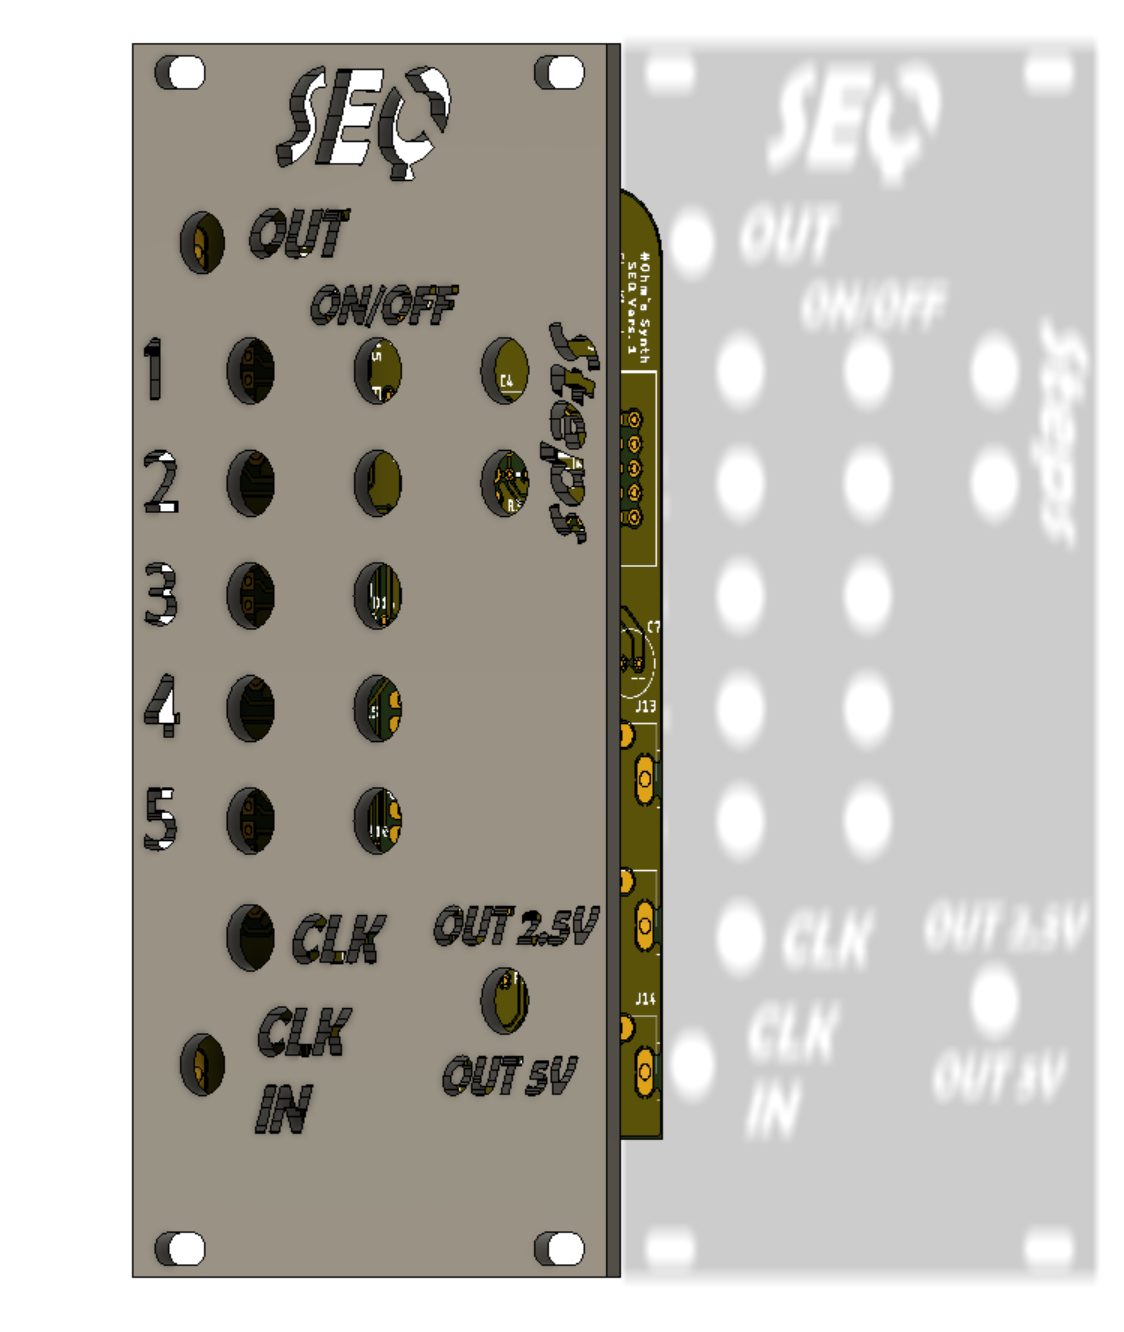
\includegraphics[width=0.6\textwidth]{figures/SEQ_Abdeckung.PNG}}
	\caption{3D-Darstellung der Sequenzer-Frontplatte}
	\label{fig:Frontplatte_SEQ}
\end{figure}
\FloatBarrier
